\documentclass[aspectratio=169, 11pt]{beamer}
\usepackage[utf8]{inputenc}
\usepackage[T1]{fontenc}
\usepackage{amsmath}
\usepackage{hyperref}
\usepackage{xcolor}
\usepackage{multicol}
\usepackage{graphicx}
\usepackage{media9}
\usepackage{tikz}

% Set the theme
\usetheme{Warsaw}

% Set the color theme
\usecolortheme{orchid}

% Set the font theme
\usefonttheme{default}

% Define a custom color 
\definecolor{myblue}{RGB}{33, 66, 99}
\definecolor{lightblue}{RGB}{80, 133, 244}
\setbeamercolor{structure}{fg=lightblue}

% Use sans serif font as default
\renewcommand{\familydefault}{\sfdefault}

% Change background color
\setbeamercolor{background canvas}{bg=white}

% Title page
\title[Sound Detection and Classification]{\textbf{Sound Detection and Classification}\\ using Spiking Neural Networks}
\author[T. Courrege, L. Gandeel]{Téo Courrege\\Loaï Gandeel}
\date{\today}


% Customize title page
\setbeamertemplate{title page}{
  \begin{centering}
    \vfill
    \textcolor{myblue}{\LARGE\inserttitle}\par
    \vspace{1cm}
    \textcolor{black}{\large\insertauthor}\par
    \vspace{1cm}
    \textcolor{black}{\small\insertdate}\par
    \vfill
  \end{centering}
}

% Customize section page
\AtBeginSection[]{
  \begin{frame}{Outline}
    \begin{multicols}{2}
      \hfill % This will push the table of contents to the right side
      \tableofcontents[currentsection, sectionstyle=show/shaded, subsectionstyle=show/show/hide]
    \end{multicols}
  \end{frame}
}


\begin{document}

\begin{frame}[plain]
  \titlepage
\end{frame}

\section{Introduction}

\begin{frame}
  \frametitle{Objectives}
  \begin{itemize}
    \item Classify audio signals using Spiking Neural Networks (SNNs).
    \item Compare the performance of SNNs with Artificial/traditional Neural Networks (ANNs).
    \item (Optional) Implement the SNNs for audio event detection (real-time processing).
  \end{itemize}
\end{frame}

\section{Theoretical Study}

\subsection{Theoretical Study of SNN}

\begin{frame}
  \frametitle{Comparison: ANN vs. SNN}
  \begin{columns}
    \begin{column}{0.5\textwidth}
      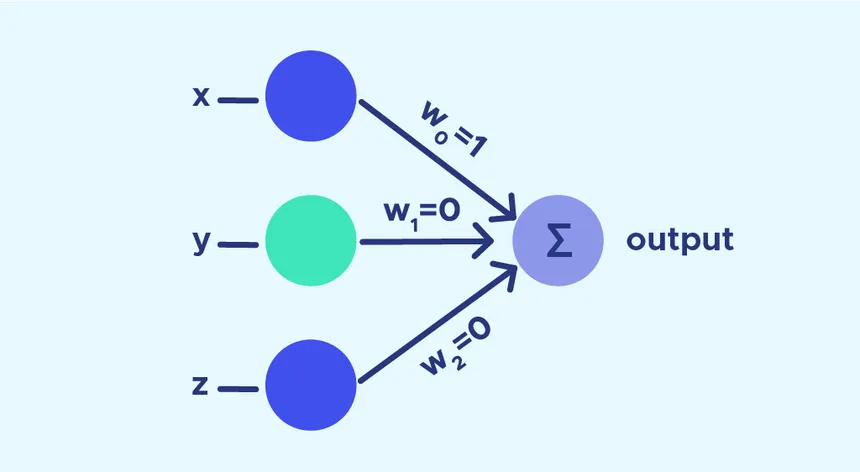
\includegraphics[width=\textwidth]{image/perceptrons.png}
    \end{column}
    \begin{column}{0.5\textwidth}
      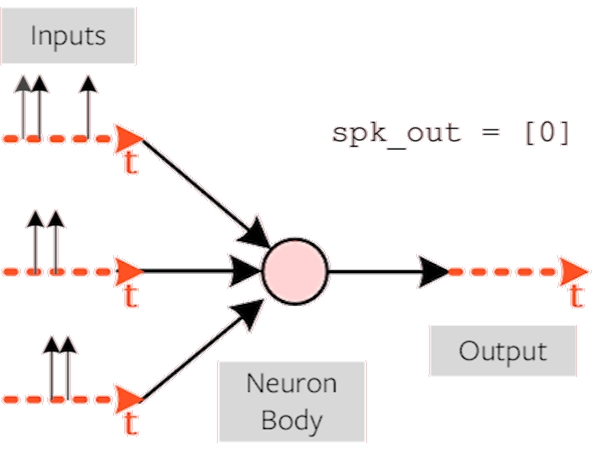
\includegraphics[width=\textwidth]{image/def1.png}
    \end{column}
  \end{columns}
\end{frame}

\begin{frame}
  \frametitle{Features of SNNs}
  \begin{itemize}
    \item Neurons communicate with each other by sending spikes.
    \item More biologically realistic than ANNs.
    \item More energy efficient than ANNs (real-time processing, event-driven processing, sparse representation).
    \item Loss function is not differentiable and cannot be optimized using gradient descent for backpropagation.
  \end{itemize}
\end{frame}

\subsection{LIF Model}
\begin{frame}
  \frametitle{Principle of LIF}
  \begin{columns}
    \begin{column}{0.5\textwidth}
      \begin{itemize}
        \item Leaky Integrate-and-Fire in SNNs
        \item Accumulates input currents over time
        \item Leaks a fraction of the charge per unit time
        \item Fires when the accumulated charge exceeds a threshold.
      \end{itemize}
    \end{column}
    \begin{column}{0.5\textwidth}
      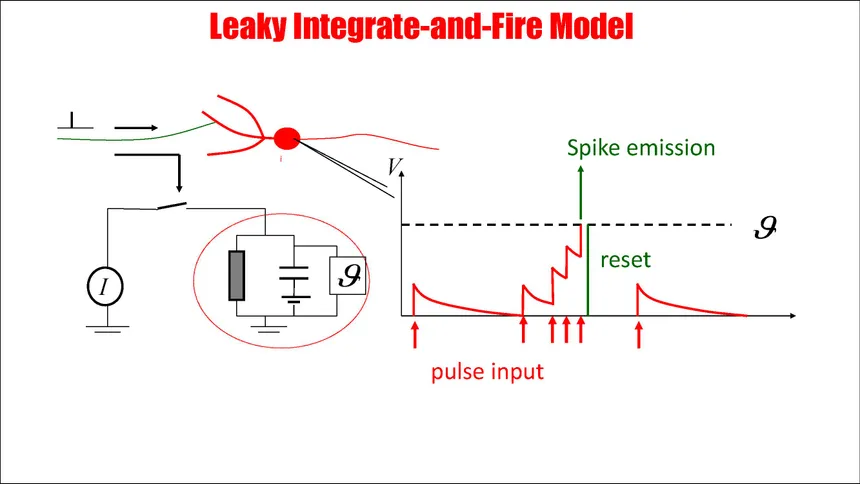
\includegraphics[width=\textwidth]{image/lif.png}
    \end{column}
  \end{columns}
\end{frame}

\begin{frame}
  \frametitle{LIF Model Equations}
  $$C_m \frac{d V_m}{d t} = I(t) - \frac{V_m}{R_m} $$
  \begin{itemize}
    \item $C_m$ is the membrane capacitance
    \item $V_m$ is the membrane potential
    \item $I(t)$ is the input current
    \item $R_m$ is the membrane resistance
  \end{itemize}
\end{frame}

\begin{frame}
  \frametitle{Comparing Spiking Neuronal Models}
  \begin{center}
    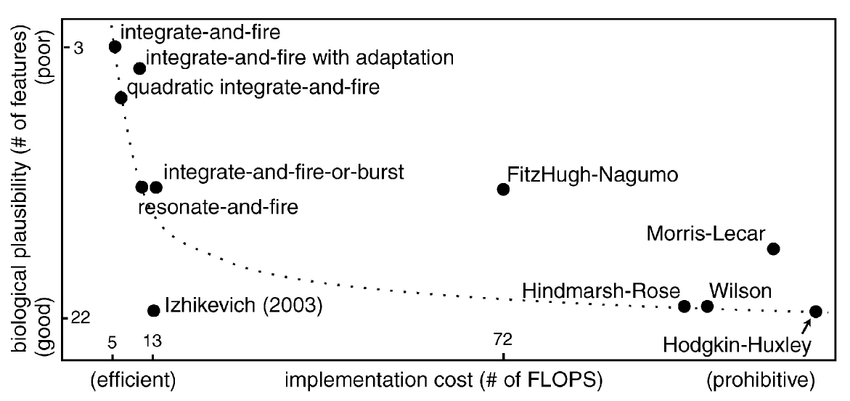
\includegraphics[width=0.8\textwidth]{image/theo1.png}
  \end{center}
\end{frame}

\section{Data, State of the Art and Pre-processing}

\subsection{Data}

\begin{frame}
  \frametitle{Audio Data}
  \begin{columns}
    \begin{column}{0.27\textwidth}
      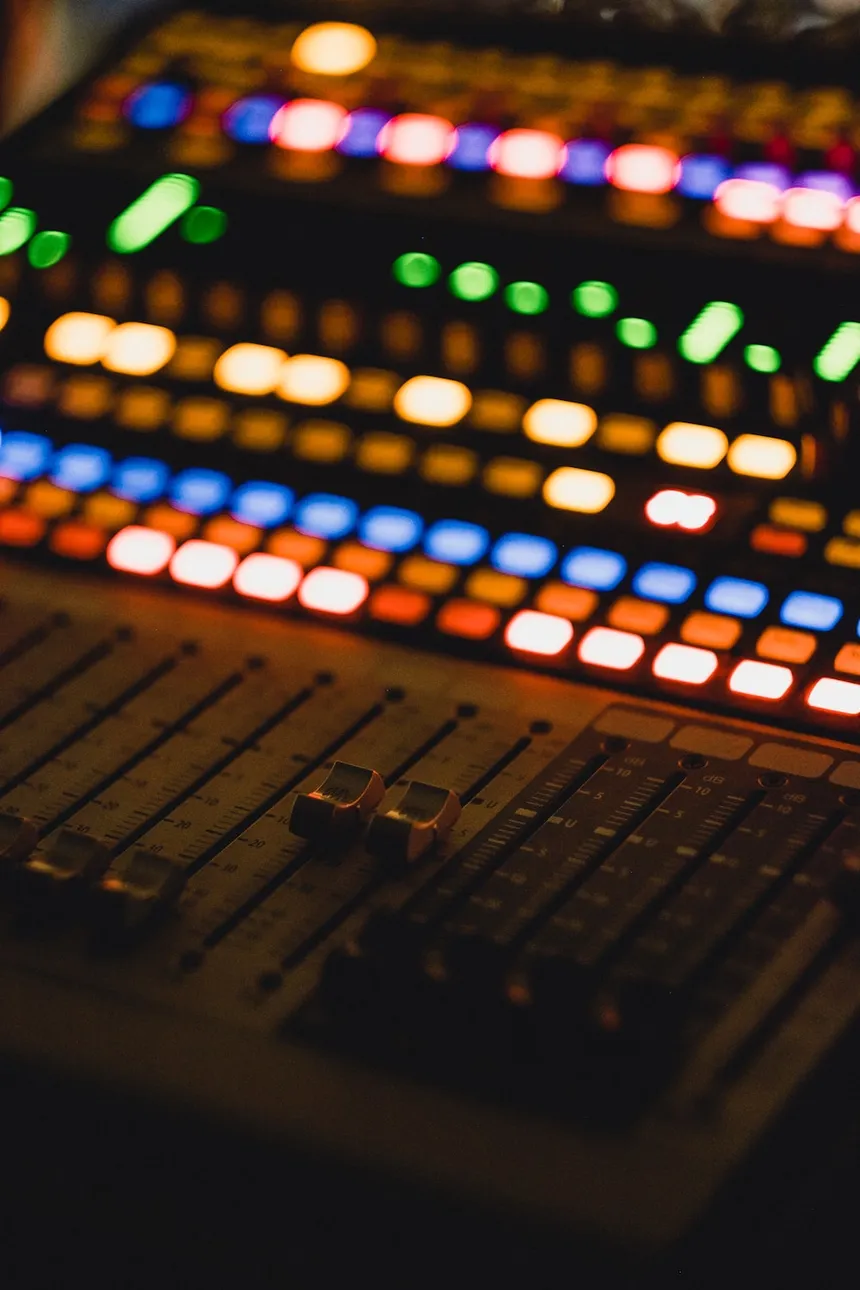
\includegraphics[width=\textwidth]{image/audio2.png}
    \end{column}
    \begin{column}{0.33\textwidth}
      
\includegraphics[width=\textwidth]{image/audio.png}
    \end{column}
    \begin{column}{0.33\textwidth}
      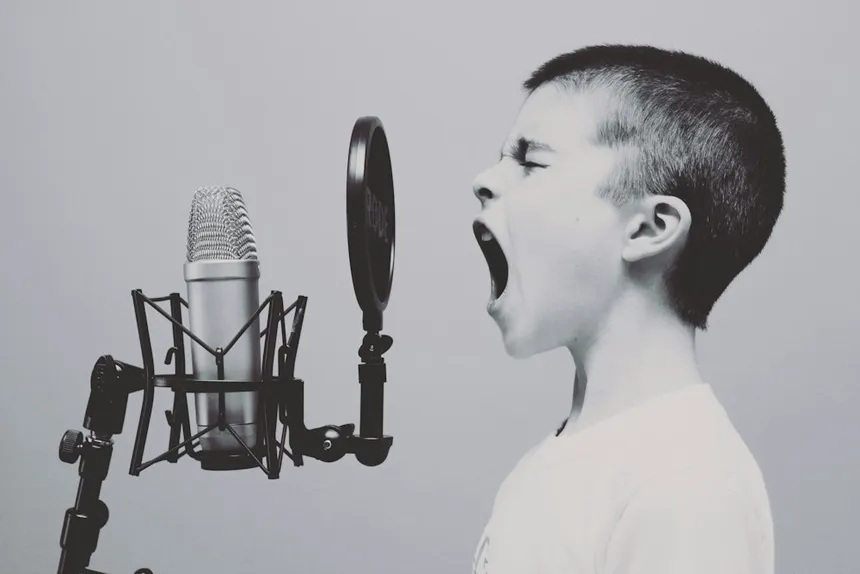
\includegraphics[width=\textwidth]{image/audio3.png}
    \end{column}
  \end{columns}
\end{frame}

\begin{frame}
  \frametitle{Google AudioSet}

  \begin{tikzpicture}[remember picture,overlay]
    \node[anchor=north east] at (current page.north east) {
\includegraphics[width=0.18\textwidth]{image/copyright.png}};
  \end{tikzpicture}

  \begin{center}
    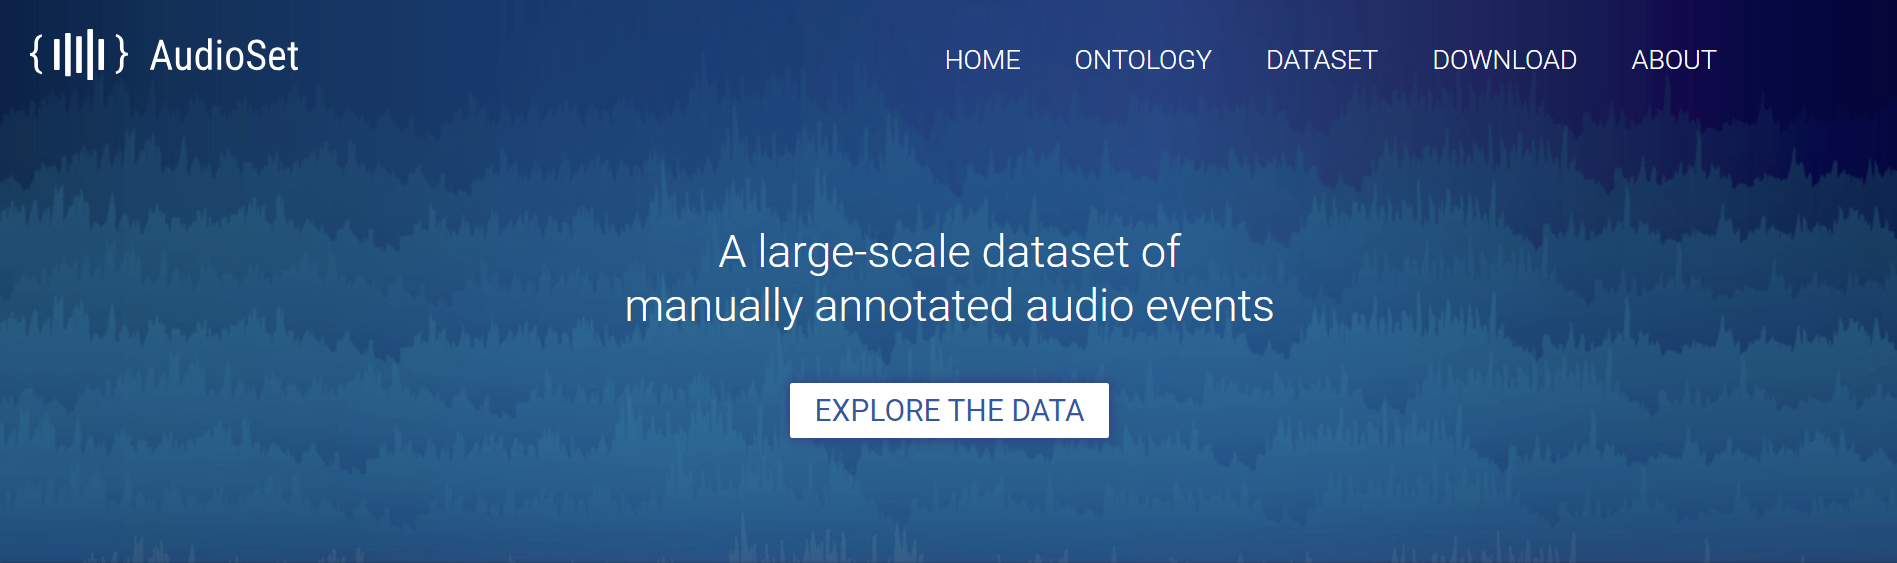
\includegraphics[width=\textwidth]{image/audioset.png}
  \end{center}

  \begin{itemize}
    \item 632 audio event classes and a collection of 2,084,320 human-labeled 10-second sound clips drawn from YouTube videos.
  \end{itemize}

\end{frame}

\subsection{State of the Art}
\begin{frame}
  \frametitle{Pretrained Models}
  \begin{itemize}
    \item  A VGG model already trained of the Google AudioSet dataset \href{https://research.google/pubs/pub45611/}{(GitHub)}.
    \item Rearanged Resnet, inception, densenet pretrained models \href{https://arxiv.org/abs/2007.11154}{(GitHub and research paper)}
    \item A spiking convolutional neural network (SCNN) for audio classification \href{https://github.com/CongSheng/SpikingConvNN-AudioClassification/tree/main}{(GitHub)}.
    \item A multi-layer SNN for audio classification using SpiNNaker \href{https://github.com/jpdominguez/Multilayer-SNN-for-audio-samples-classification-using-SpiNNaker}{(GitHub)}.
  \end{itemize}

\end{frame}

\subsection{Pre-processing}

\begin{frame}
  \frametitle{Dataset Challenges}

  \begin{columns}
    \begin{column}{0.1\textwidth} % adjust the width as needed
      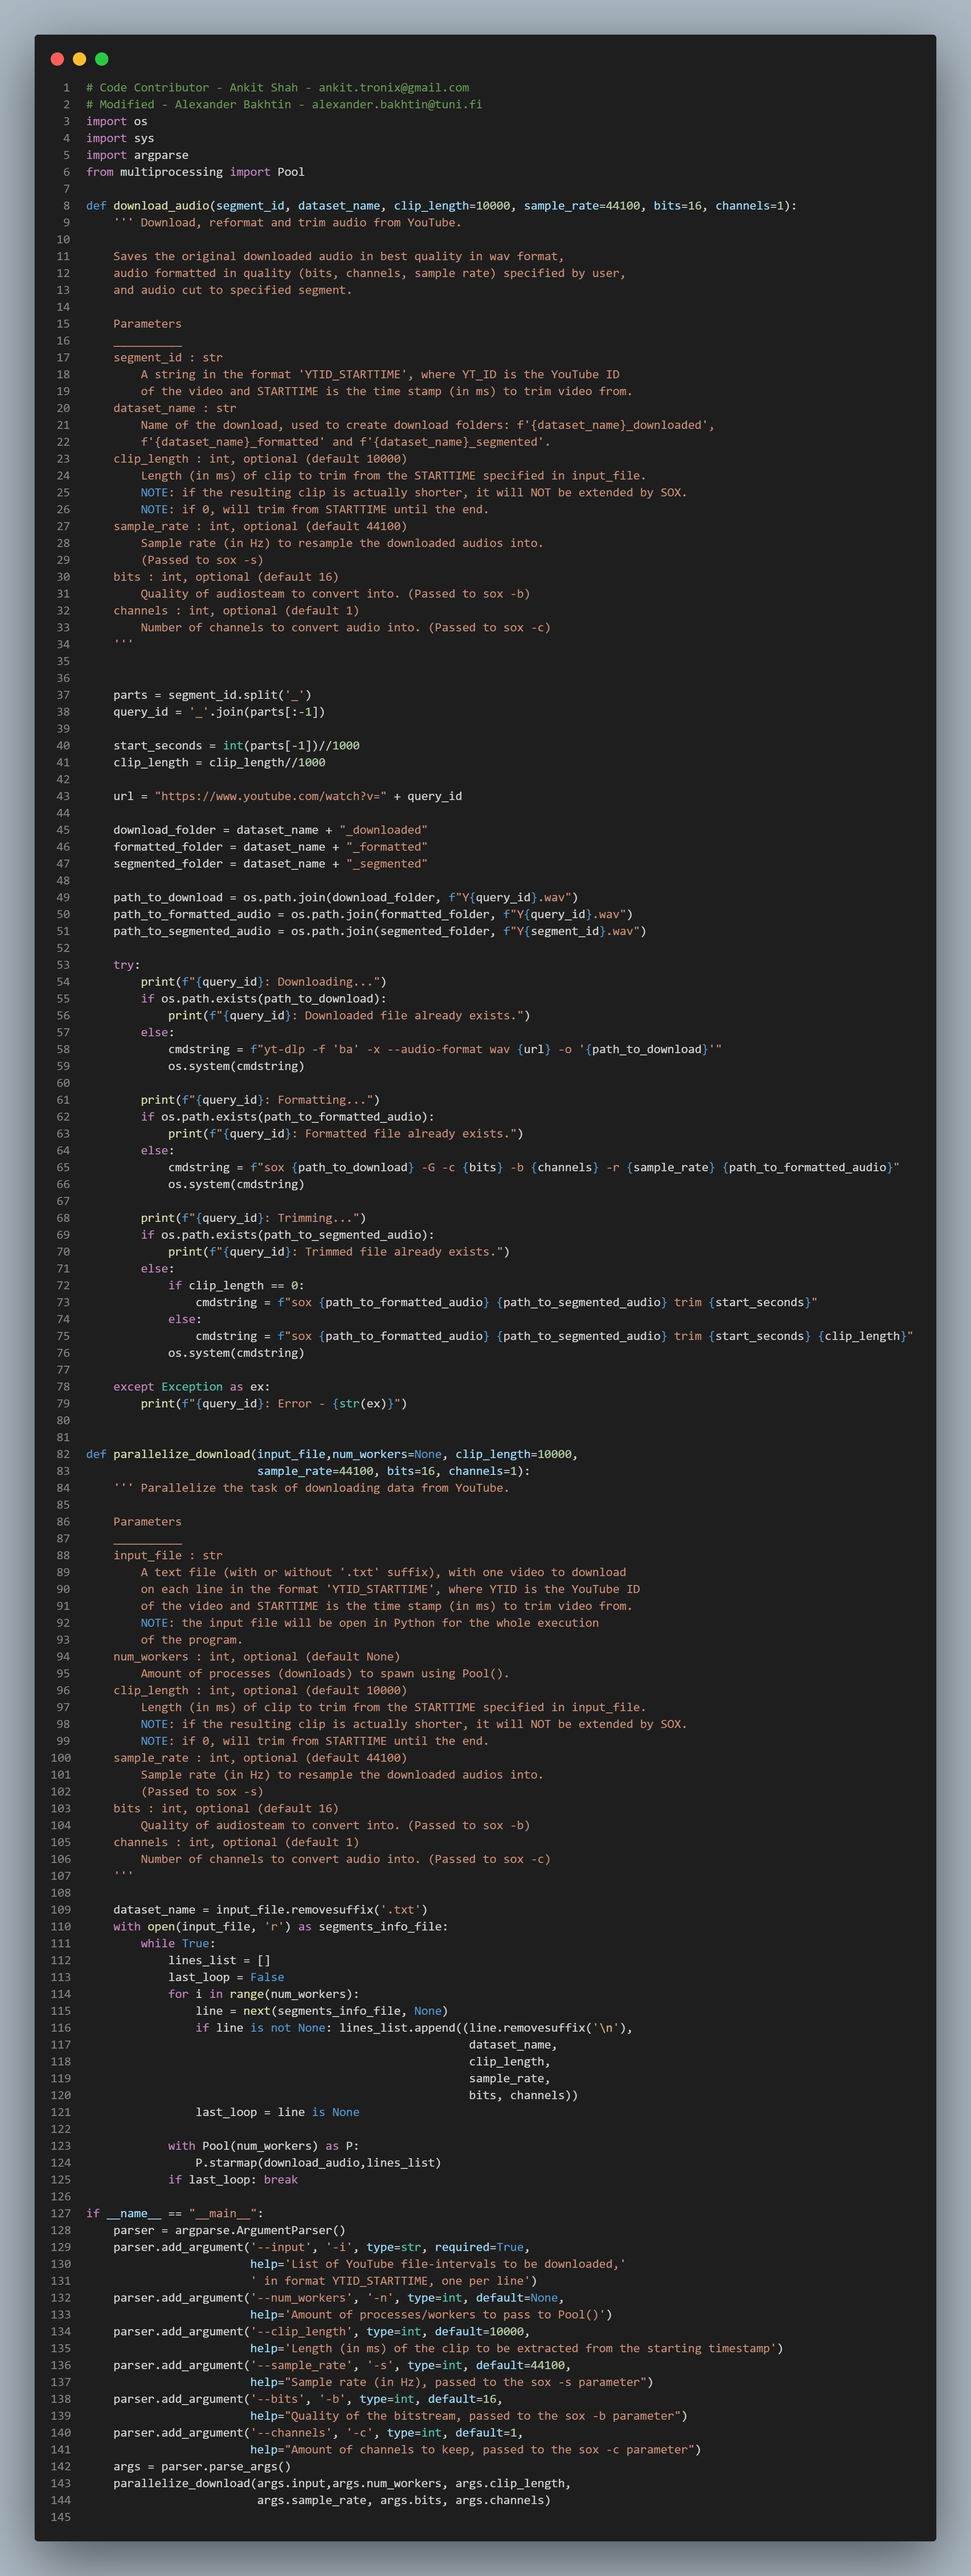
\includegraphics[width=\textwidth]{image/short_code.png}
    \end{column}

    \begin{column}{0.05\textwidth} % adjust the width as needed

    \end{column}

    \begin{column}{0.1\textwidth} % adjust the width as needed
      % leave this column empty or add content as needed
    \end{column}
  \end{columns}

\end{frame}



\begin{frame}
  \frametitle{Dataset Challenges}

  \begin{columns}
    \begin{column}{0.1\textwidth} % adjust the width as needed
      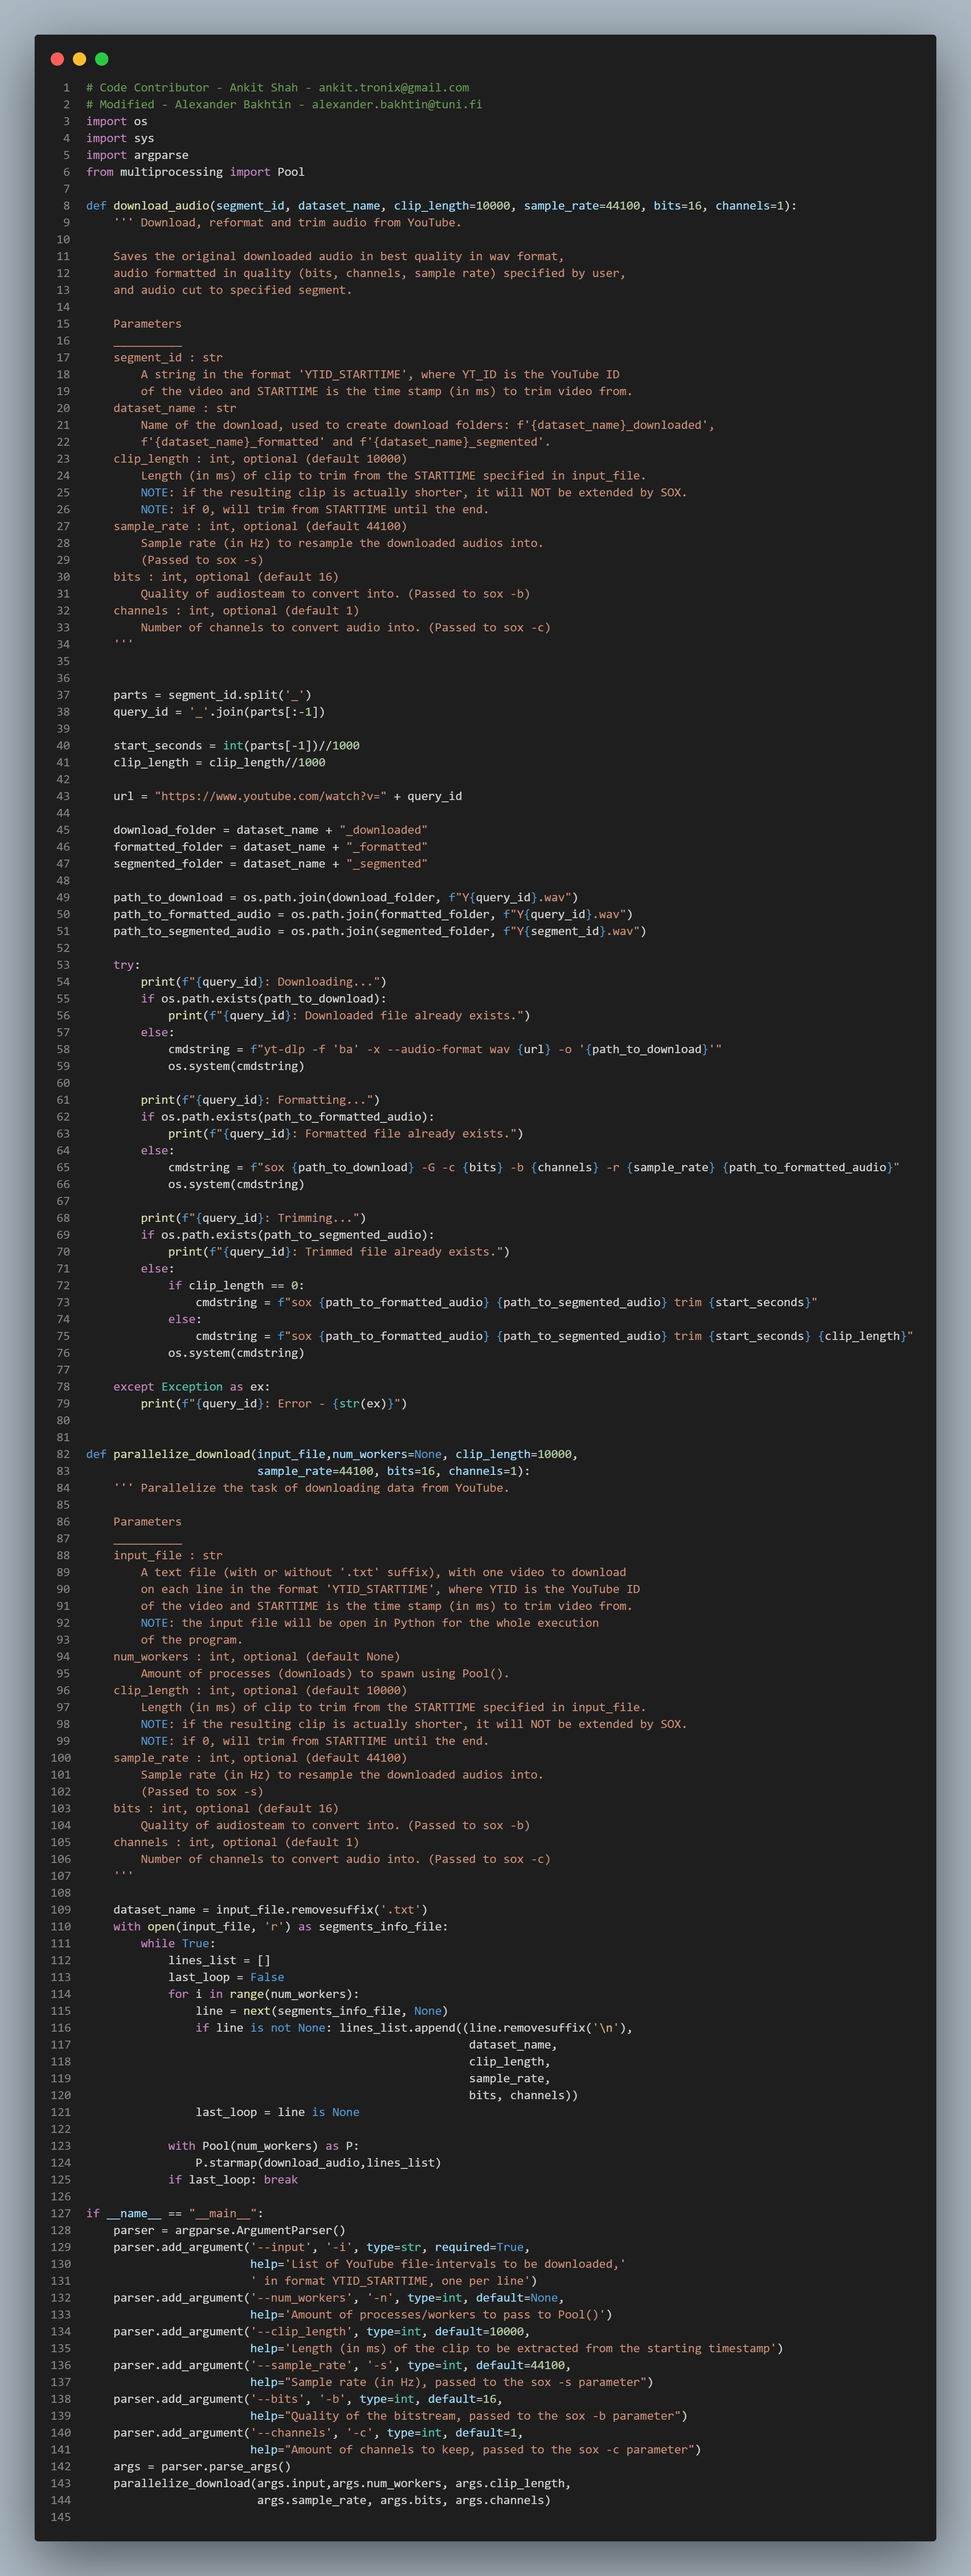
\includegraphics[width=\textwidth]{image/short_code.png}
    \end{column}

    \begin{column}{0.05\textwidth} % adjust the width as needed
      \centering
      \scalebox{2.0}{$\rightarrow$} % scale the arrow to be twice as big
    \end{column}

    \begin{column}{0.1\textwidth} % adjust the width as needed
      
\includegraphics[width=\textwidth]{image/long_code.png}
    \end{column}
  \end{columns}
\end{frame}

\begin{frame}
  \frametitle{Dataset Challenges}
  \begin{itemize}
    \item Collect enough data to train a model as efficiently as possible.
    \item Format all audio files in the same way.
    \item Parallelize the hole process.
    \item Make sure there are no errors or anomalies.
    \item Check for redundancies in the labels associated with the audio files (avoid unbalanced data).
  \end{itemize}
\end{frame}

\section{Spectrograms, MEL and MFCC}

\subsection{Spectrogram}

\begin{frame}{Spectrograms}
  \begin{center}
    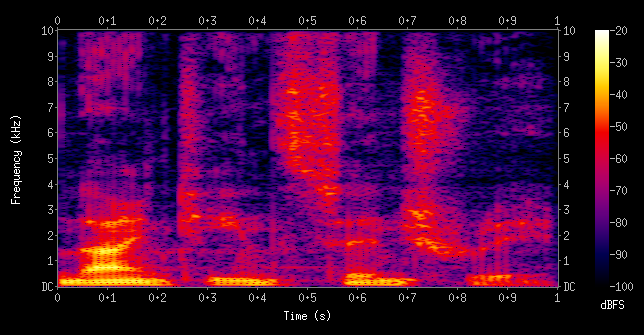
\includegraphics[width=0.8\textwidth]{image/Spectrogram.png}
  \end{center}
\end{frame}

\subsection{MEL spectrogram}

\begin{frame}{MEL}
  \begin{center}
    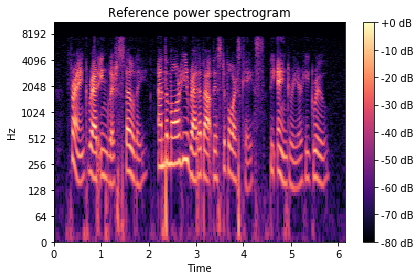
\includegraphics[width=0.7\textwidth]{image/Mel_spectro.png}
  \end{center}
\end{frame}

\subsection{Mel Frequency Cepstral Coefficients}

\begin{frame}{MFCC}
  \begin{center}
    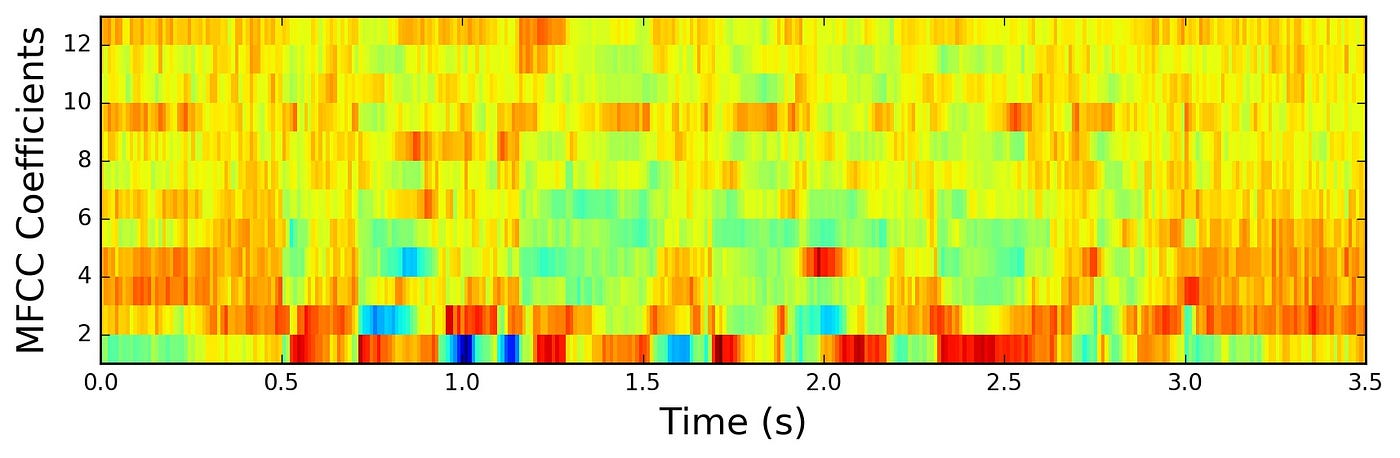
\includegraphics[width=\textwidth]{image/mfcc.jpg}
  \end{center}
\end{frame}

\section{Results}

\subsection{Original Audio}

\begin{frame}{Original Audio}
  \begin{columns}
    \begin{column}{0.5\textwidth}
      \centering
      \includemedia[
        addresource=audio/piano_original.wav,
        flashvars={
            source=audio/piano_original.wav
            &autoPlay=false
            &hideBar=false
          },
      ]{\fbox{Play}}{APlayer.swf}
    \end{column}
    \begin{column}{0.5\textwidth}
      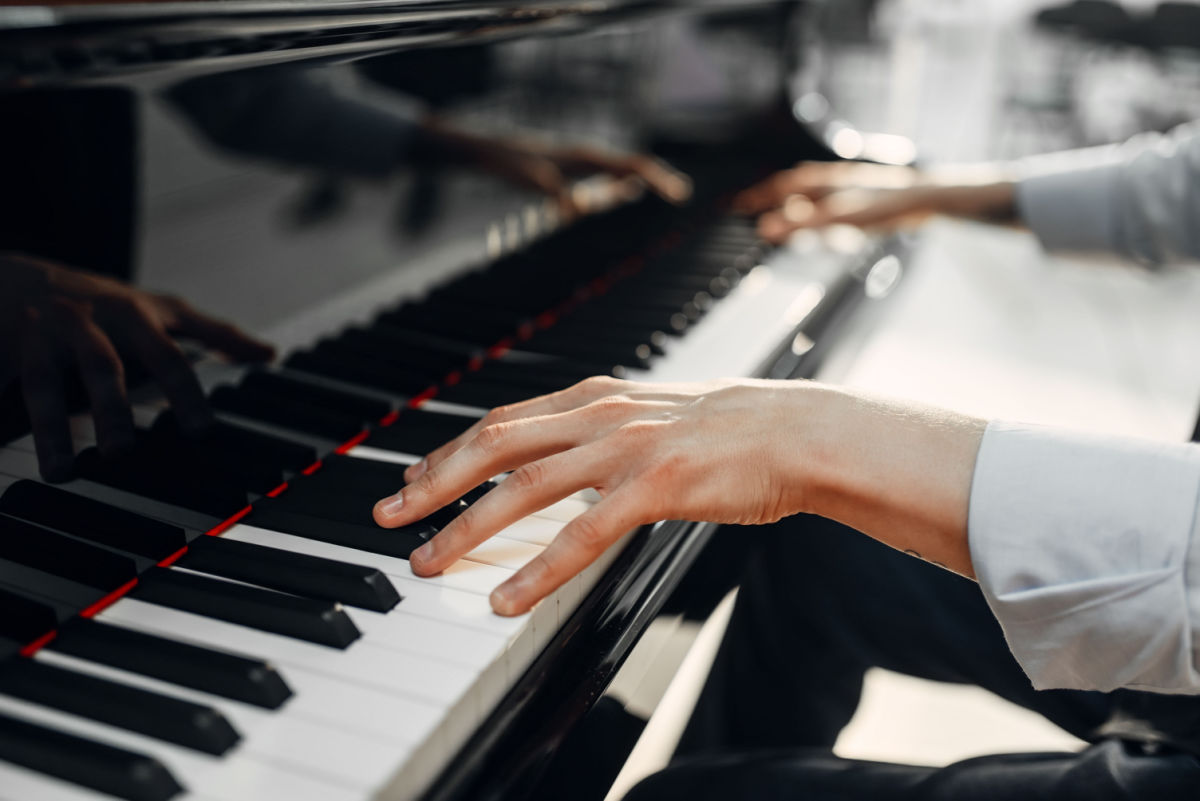
\includegraphics[width=\textwidth]{image/piano.png}
    \end{column}
  \end{columns}
\end{frame}

\subsection{MFCC reconstruction}

\begin{frame}{MFCC reconstruction}
  \begin{columns}
    \begin{column}{0.5\textwidth}
      \centering
      \includemedia[
        addresource=audio/piano_mfcc_reconstruction.wav,
        flashvars={
            source=audio/piano_mfcc_reconstruction.wav
            &autoPlay=false
            &hideBar=false
          },
      ]{\fbox{Play}}{APlayer.swf}
    \end{column}
    \begin{column}{0.5\textwidth}
      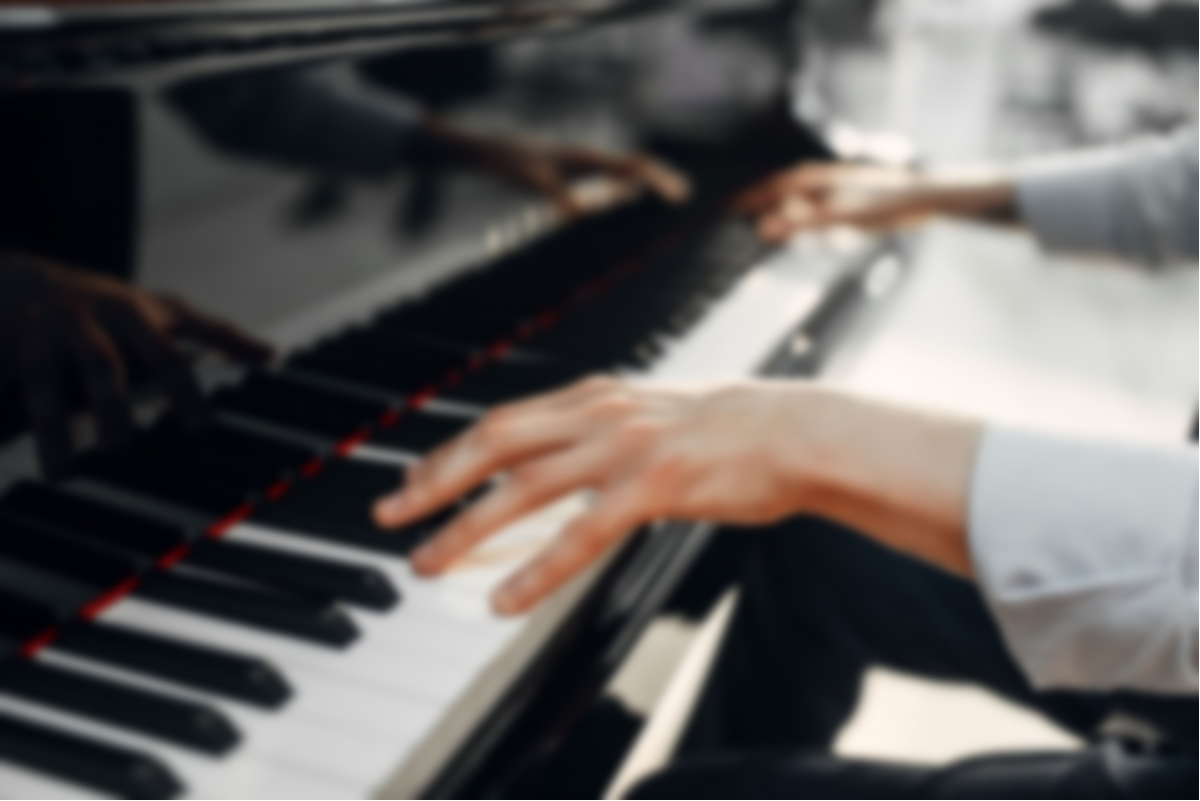
\includegraphics[width=\textwidth]{image/piano_blur1.png}
    \end{column}
  \end{columns}
\end{frame}

\subsection{Latency reconstruction}

\begin{frame}{Latency reconstruction}
  \begin{columns}
    \begin{column}{0.5\textwidth}
      \centering
      \includemedia[
        addresource=audio/piano_latency_reconstruction.wav,
        flashvars={
            source=audio/piano_latency_reconstruction.wav
            &autoPlay=false
            &hideBar=false
          },
      ]{\fbox{Play}}{APlayer.swf}
    \end{column}
    \begin{column}{0.5\textwidth}
      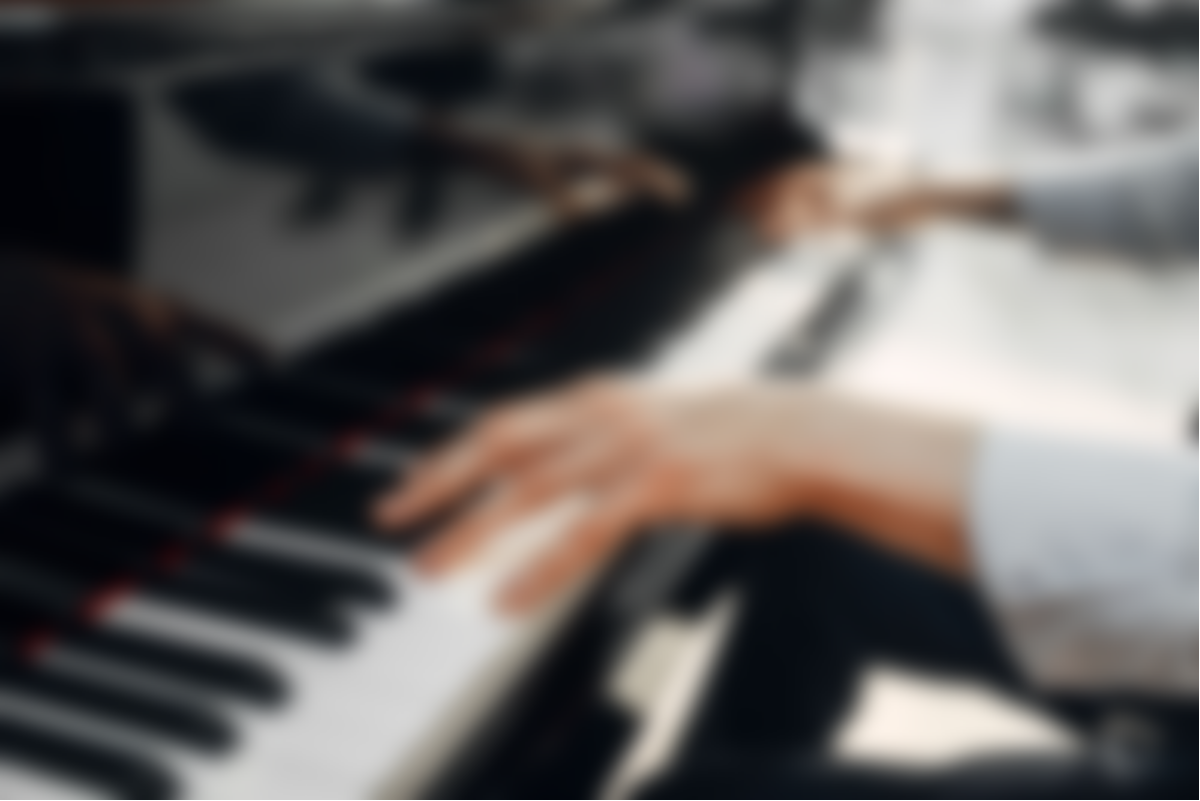
\includegraphics[width=\textwidth]{image/piano_blur2.png}
    \end{column}
  \end{columns}
\end{frame}

\subsection{Rate reconstruction}

\begin{frame}{Rate reconstruction}
  \begin{columns}
    \begin{column}{0.5\textwidth}
      \centering
      \includemedia[
        addresource=audio/piano_rate_reconstruction.wav,
        flashvars={
            source=audio/piano_rate_reconstruction.wav
            &autoPlay=false
            &hideBar=false
          },
      ]{\fbox{Play}}{APlayer.swf}
    \end{column}
    \begin{column}{0.5\textwidth}
      
\includegraphics[width=\textwidth]{image/piano_blur3.png}
    \end{column}
  \end{columns}
\end{frame}

\section{Conclusion}

\subsection{Achievements and Future Work}
\begin{frame}{Conclusion}
  Achievements:
  \begin{itemize}
    \item "Usuable and balanced" dataset.
    \item Knowledge on the encoding a decoding of audio signals into spikes.
  \end{itemize}
  Future work:
  \begin{itemize}
    \item Implement a simple architecture SNN for audio classification (2 - 5 days of work)
    \item Implement the pretrained ANN models for comparison (2 - 5 days of work)
  \end{itemize}
\end{frame}

\subsection*{prompt : "Spiking Neural Networks"}

\begin{frame}
  \frametitle{Funny images}

  \begin{columns}
    \begin{column}{0.5\textwidth} % adjust the width as needed
      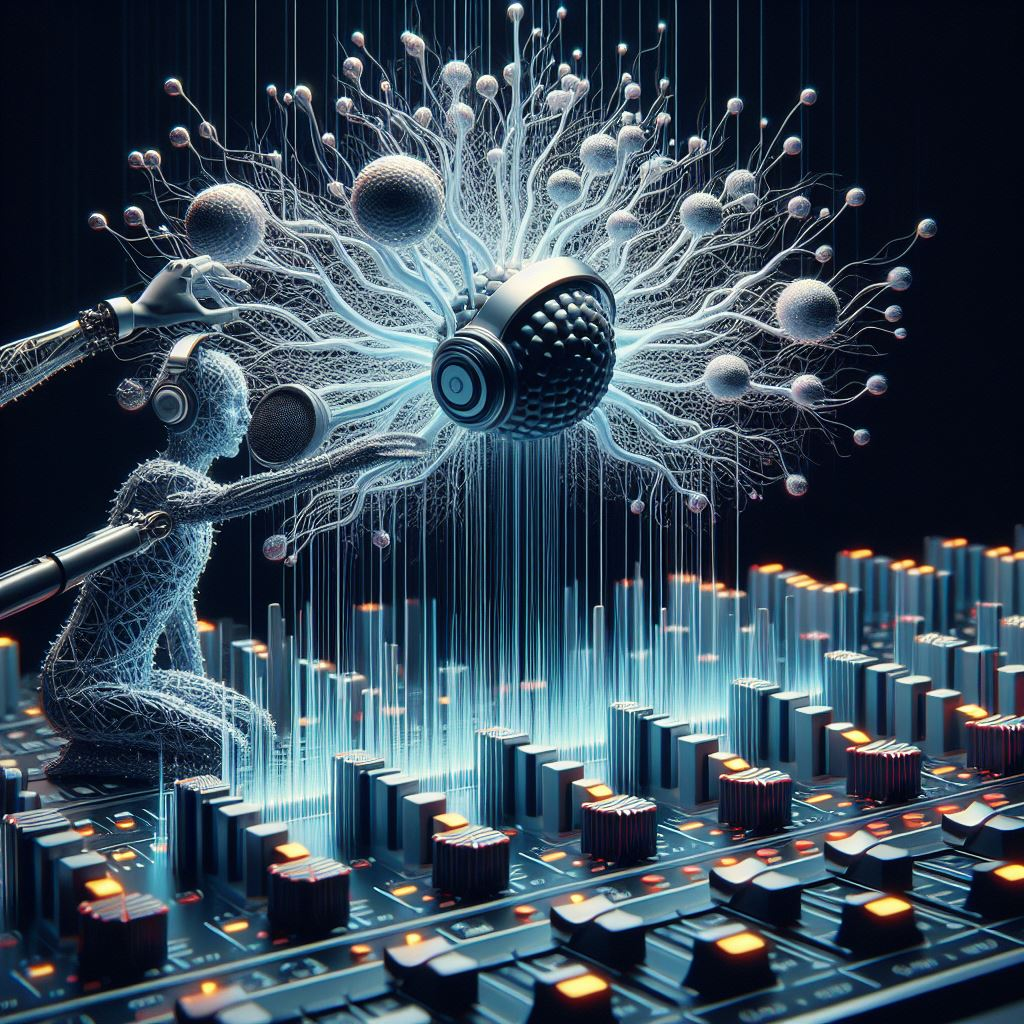
\includegraphics[width=\textwidth]{image/2.jpeg}
    \end{column}

    \begin{column}{0.5\textwidth} % adjust the width as needed
      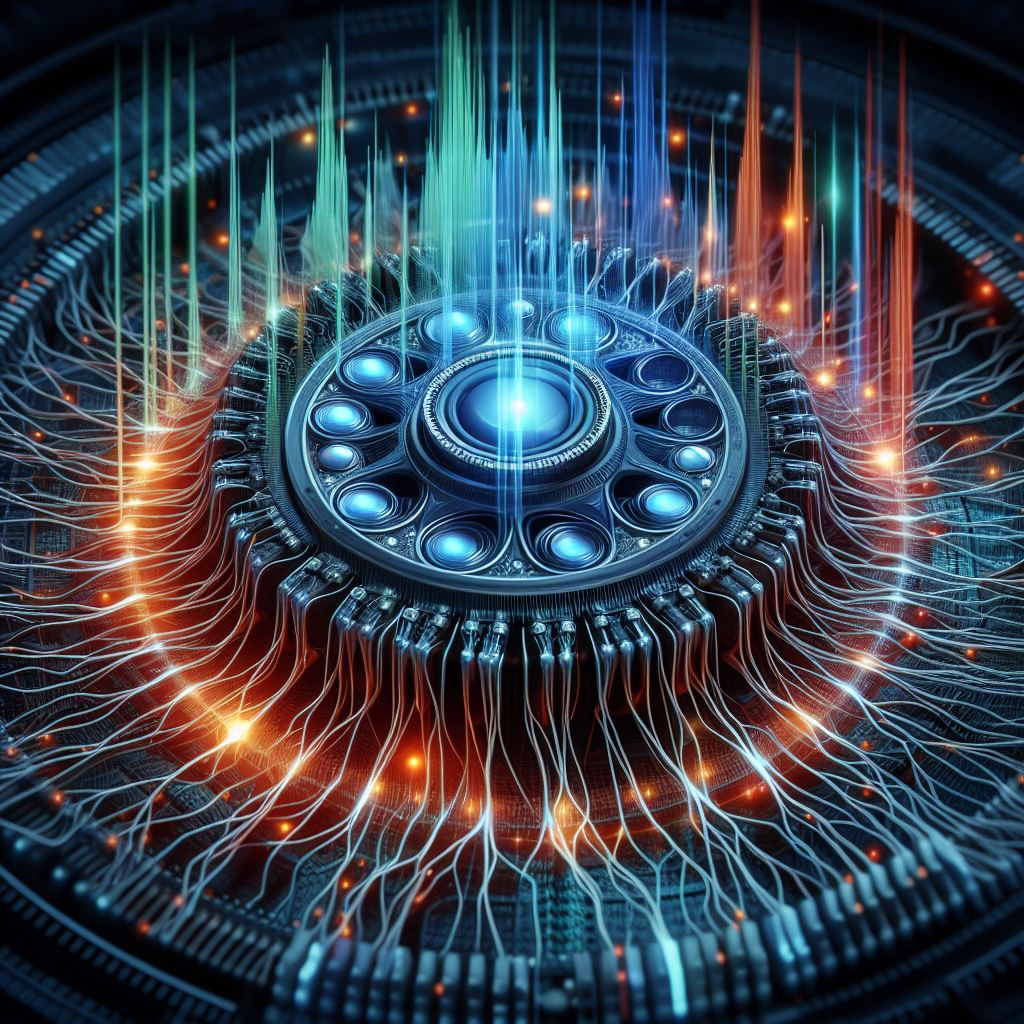
\includegraphics[width=\textwidth]{image/1.jpeg}
    \end{column}
  \end{columns}
\end{frame}

\subsection*{prompt : "Spiking Neural Networks for audio classification"}

\begin{frame}
  \frametitle{Funny images}

  \begin{columns}
    \begin{column}{0.5\textwidth} % adjust the width as needed
      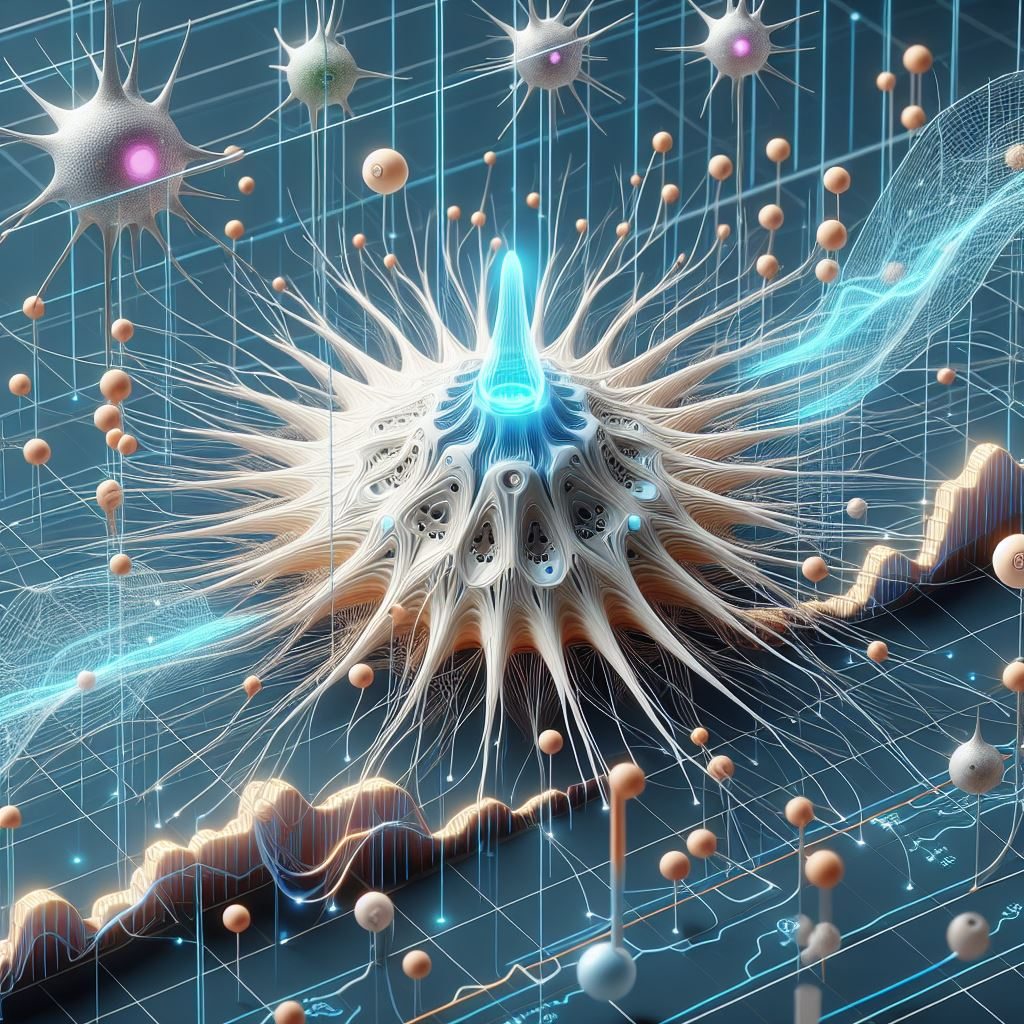
\includegraphics[width=\textwidth]{image/3.jpeg}
    \end{column}

    \begin{column}{0.5\textwidth} % adjust the width as needed
      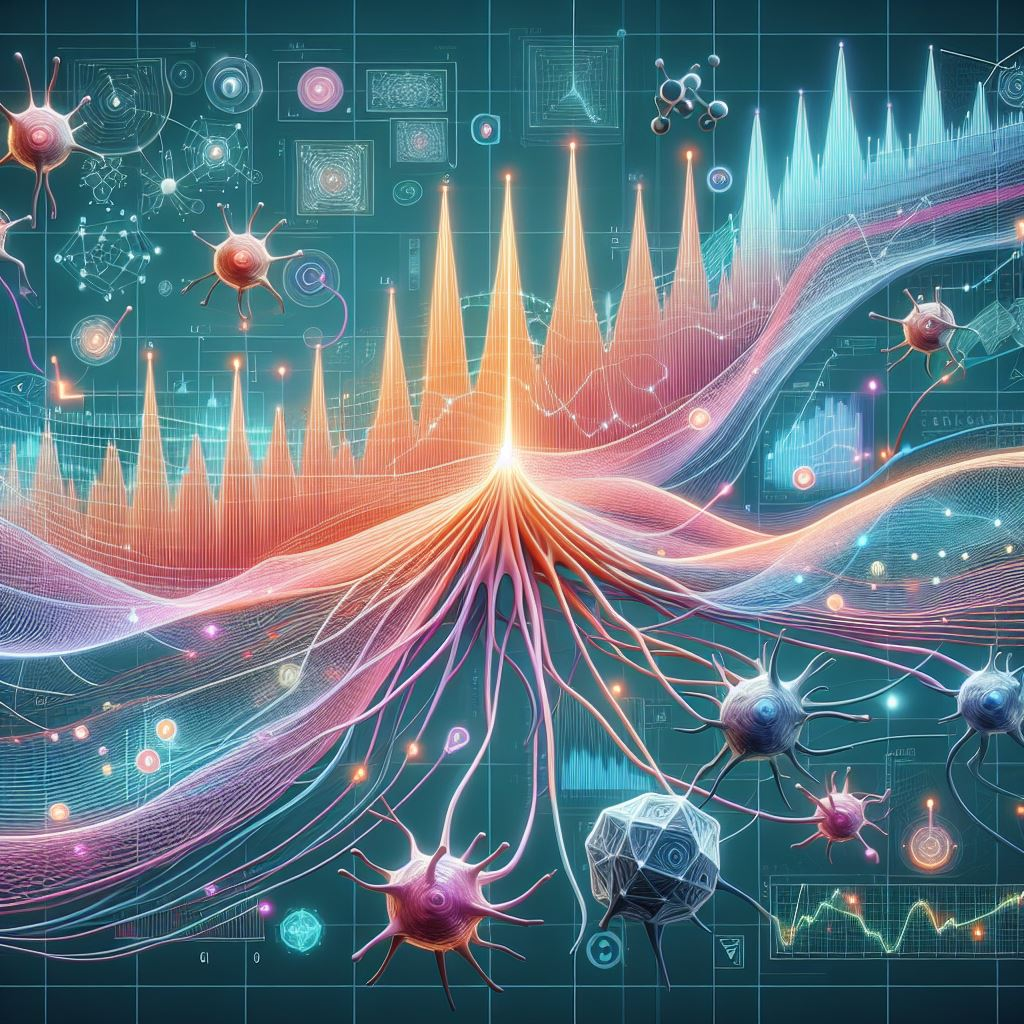
\includegraphics[width=\textwidth]{image/4.jpeg}
    \end{column}
  \end{columns}
\end{frame}

\end{document}
